\documentclass[11pt]{article}

\usepackage[most]{tcolorbox}
\usepackage{luatexja}
\usepackage{array}
\usepackage[margin=25mm]{geometry}

%セルの長さを指定して縦にそろえる
\newcolumntype{M}[1]{>{\centering\arraybackslash}m{#1}}

\setlength{\parindent}{0pt}
\linespread{1.2} %行間を調整

%tcolorboxのスタイルを設定
\tcbset{
  mybox/.style={
    %colback=yellow!5,
    %colframe=orange!80!black,
    fonttitle=\bfseries,
    title=#1
  }
}

\begin{document}

\begin{tcolorbox}[mybox={直線}]
2点を線で結ぶことを考える。2点を結ぶように両方向に伸ばした線を\textbf{直線}という。\\
2点の間を線で結んだ線を\textbf{線分}という。一方向だけに伸ばした線を\textbf{半直線}という。\\
点$A$と点$B$を通る直線を、\textbf{直線$AB$}と呼ぶ。線分や半直線についても同じ。\\

\begin{tikzpicture}
%直線
\coordinate (P1) at (0,0);
\coordinate (A1) at (1,0);
\coordinate (B1) at (3,0);
\coordinate (Q1) at (4,0);
\draw[thick] (P1)--(Q1);
\fill[blue] (A1) circle (2pt);
\fill[blue] (B1) circle (2pt);
\node[xshift=0pt, below=5pt] at (A1) {A};
\node[xshift=0pt, below=5pt] at (B1) {B};
\node at (2,1) {直線AB};

%線分
\coordinate (A2) at (6,0);
\coordinate (B2) at (9,0);
\draw[thick] (A2)--(B2);
\fill[blue] (A2) circle (2pt);
\fill[blue] (B2) circle (2pt);
\node[xshift=0pt, below=5pt] at (A2) {A};
\node[xshift=0pt, below=5pt] at (B2) {B};
\node at (7.5,1) {線分AB};

%半直線
\coordinate (A3) at (11,0);
\coordinate (B3) at (14,0);
\coordinate (Q3) at (15.5,0);
\draw[thick] (A3)--(Q3);
\fill[blue] (A3) circle (2pt);
\fill[blue] (B3) circle (2pt);
\node[xshift=0pt, below=5pt] at (A3) {A};
\node[xshift=0pt, below=5pt] at (B3) {B};
\node at (12.5,1) {半直線AB};
\end{tikzpicture}
\end{tcolorbox}

\bigskip

点や直線に、アルファベットで名前をつけます。その理由は、、、\\

図の中に点や直線がたくさんあったときに、どの点や直線のことを説明しているか混乱しやすいです。そのため、点や直線に名前を付けることが多いです。名前をつけることで、はっきりと説明ができます。\\

名前としては、A,B,Cなどのアルファベットで名前をつけます。\\
\begin{center}
\begin{tikzpicture}
\coordinate (A) at (1,1);
\node[below=3pt] at (A) {A};
\fill[black] (A) circle (2pt);
\draw[thick] (4,0)--(8,1);
\node at (6,1) {L};
\end{tikzpicture}
\end{center}

%長さが同じ記号と中点
\begin{tcolorbox}[mybox={中点}]
線分の真ん中の点を\textbf{中点}という。\\

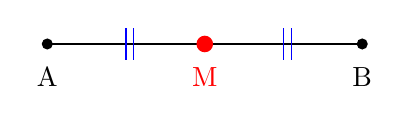
\begin{tikzpicture}
\coordinate (A) at (0,0);
\coordinate (B) at (4,0);
\coordinate (M) at (2,0);
\draw[thick] (A)--(B);
\fill[black] (A) circle (2pt);
\fill[black] (B) circle (2pt);
\fill[red] (M) circle (3pt);
\node[xshift=0pt, below=5pt] at (A) {A};
\node[xshift=0pt, below=5pt] at (B) {B};
\node[xshift=0pt, below=5pt,red] at (M) {M};
%同じ長さの記号
\draw[blue] (1,0.2)--(1,-0.2);
\draw[blue] (1.1,0.2)--(1.1,-0.2);
\draw[blue] (3,0.2)--(3,-0.2);
\draw[blue] (3.1,0.2)--(3.1,-0.2);
\end{tikzpicture}
\end{tcolorbox}

%角をアルファベットで表す
%角度が同じ記号
\begin{tcolorbox}[mybox={角と三角形}]
三角形の記号は反時計回りにつける。\\

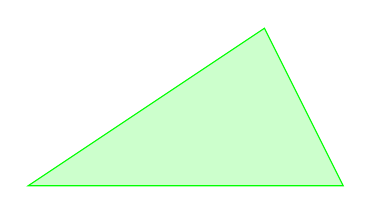
\begin{tikzpicture}
\draw[green,fill=green!20!white] (0,0)--(4,0)--(3,2)--cycle;
\end{tikzpicture}
\end{tcolorbox}

%直線の位置関係
\begin{tcolorbox}[mybox={垂直と平行}]
2つの直線が交わらないとき、2つの直線は\textbf{平行}という\\
1つの直線にもう一つの直線が直角に交わるとき、直線は\textbf{垂直}であるという\\
線分に垂直に交わり、中点を通る直線を\textbf{垂直二等分線}という。\\

\begin{tikzpicture}
\draw[thick] (0,-1)--(3,0);
\draw[thick,red] (0,0)--(3,1);
\draw[thick] (5,0)--(9,0);
\draw[thick,blue] (7,1.5)--(7,-1.5);
\draw[blue] (7,0.25)--(7.25,0.25)--(7.25,0);
\end{tikzpicture}
\end{tcolorbox}

\begin{tcolorbox}[mybox={距離}]
a
\end{tcolorbox}

\end{document}